% Thanksgiving
% Compile with: latexmk -pdf thanksgiving.tex
\documentclass[aspectratio=169,11pt]{beamer}

\usepackage[T1]{fontenc}
\usepackage{lmodern}
\usepackage{booktabs}
\usepackage{array}
\usepackage{tikz}
\usetikzlibrary{shapes.geometric,positioning,calc,arrows.meta}
\usepackage{pgfplots}
\pgfplotsset{compat=1.18}
\usepackage[most]{tcolorbox}
\graphicspath{{images/}}

% ---------- Colors ----------
\definecolor{navy}{HTML}{1C2541}
\definecolor{oldred}{HTML}{B22234}   % US flag red, also the accent color
\definecolor{oldblue}{HTML}{3C3B6E}  % US flag blue
\definecolor{ink}{HTML}{2B2B2B}
\definecolor{muted}{HTML}{8A8F98}
\definecolor{paper}{HTML}{FFFFFF}
\definecolor{dem}{HTML}{2E5FA3}      % Democrats
\definecolor{rep}{HTML}{C0392B}      % Republicans
\definecolor{austria}{HTML}{C8102E}  % Austria red, for USA-vs-Austria comparisons

% ---------- Minimal theme ----------
\setbeamertemplate{navigation symbols}{}
\setbeamercolor{normal text}{fg=ink, bg=paper}
\setbeamercolor{structure}{fg=navy}
\setbeamercolor{frametitle}{fg=navy}
\setbeamercolor{alerted text}{fg=oldred}
\setbeamercolor{footnote}{fg=muted}
\setbeamerfont{frametitle}{size=\Large, series=\bfseries}
\setbeamertemplate{itemize item}{\color{oldred}\textbullet}
\setbeamertemplate{itemize subitem}{\color{muted}--}
\setbeamertemplate{enumerate item}{\color{oldred}\insertenumlabel.}
\setbeamersize{text margin left=1.1cm, text margin right=1.1cm}
\hypersetup{colorlinks=true, urlcolor=dem, linkcolor=navy}

\setbeamertemplate{frametitle}{%
  \vspace*{0.5cm}%
  \usebeamerfont{frametitle}\usebeamercolor[fg]{frametitle}\insertframetitle\par
  \vspace{0.15cm}{\color{navy!15}\rule{\textwidth}{0.4pt}}\par}

\setbeamertemplate{footline}{%
  \hfill{\tiny\color{muted}\insertframenumber}\hspace*{0.6cm}\vspace*{0.35cm}}

% Plain divider at the start of each section
\AtBeginSection{%
  \begin{frame}[plain,noframenumbering]
    \centering
    {\LARGE\bfseries\color{navy}\insertsection}\\[0.6em]
    {\color{oldred}\rule{1.5cm}{0.8pt}}
  \end{frame}}

% "Think" question slides: \begin{thinkframe} ... \end{thinkframe}
\newenvironment{thinkframe}{%
  \begin{frame}[plain,noframenumbering,environment=thinkframe]\centering\Large}{\end{frame}}

% ---------- Helpers ----------
% Small grey source line at the bottom of a frame
\newcommand{\source}[1]{%
  \begin{tikzpicture}[remember picture,overlay]
    \node[anchor=south west, font=\tiny, text=muted, text width=0.85\paperwidth, align=left]
      at ($(current page.south west)+(0.6cm,0.25cm)$) {#1};
  \end{tikzpicture}}

% Quote box with a thin red rule on the left; optional arg e.g. [fontupper=\itshape\small]
\newtcolorbox{textquote}[1][]{%
  enhanced, frame hidden, boxrule=0pt, sharp corners,
  colback=navy!4, borderline west={2pt}{0pt}{oldred},
  left=10pt, right=8pt, top=6pt, bottom=6pt, fontupper=\itshape, #1}

% Photo + name + short bio (use inside a column): \candidate{file}{Name}{bio}
\newcommand{\candidate}[3]{%
  \begin{minipage}[t]{\linewidth}\centering
    \includegraphics[height=3.5cm]{#1}\\[0.5em]
    {\large\bfseries\color{navy}#2}\\[0.4em]
    \begin{minipage}{0.9\linewidth}\raggedright\small #3\end{minipage}
  \end{minipage}}

% Big number with a caption (use inside a column): \bignum{color}{91\%}{caption}
\newcommand{\bignum}[3]{%
  \begin{minipage}[t]{\linewidth}\centering
    {\fontsize{34}{38}\selectfont\bfseries\color{#1}#2}\\[0.3em]
    {\small #3}
  \end{minipage}}

% US flag drawn in TikZ (hoist height = #1), e.g. \usflag{3cm}
\newcommand{\usflag}[1]{%
  \begin{tikzpicture}[x=#1, y=#1]
    \def\fly{1.9}
    \foreach \i in {0,...,12} {
      \pgfmathsetmacro{\c}{mod(\i,2)==0 ? 1 : 0}
      \ifdim\c pt=1pt
        \fill[oldred] (0,{1-(\i+1)/13}) rectangle (\fly,{1-\i/13});
      \else
        \fill[white] (0,{1-(\i+1)/13}) rectangle (\fly,{1-\i/13});
      \fi
    }
    \def\cw{0.76} \def\ch{0.5385}
    \fill[oldblue] (0,{1-\ch}) rectangle (\cw,1);
    \foreach \r in {1,...,9} {
      \pgfmathsetmacro{\isodd}{mod(\r,2)}
      \ifdim\isodd pt=1pt
        \foreach \k in {0,...,5}
          \node[star, star points=5, star point ratio=2.618, fill=white, inner sep=0pt,
                minimum size=0.0616*#1] at ({(2*\k+1)*\cw/12},{1-\r*\ch/10}) {};
      \else
        \foreach \k in {0,...,4}
          \node[star, star points=5, star point ratio=2.618, fill=white, inner sep=0pt,
                minimum size=0.0616*#1] at ({(2*\k+2)*\cw/12},{1-\r*\ch/10}) {};
      \fi
    }
    \draw[ink!30, line width=0.3pt] (0,0) rectangle (\fly,1);
  \end{tikzpicture}}

% Agree/disagree spectrum for "spectrum game" activities
\newcommand{\spectrum}{%
  
\begin{tikzpicture}
    \shade[left color=oldblue, right color=oldred, rounded corners=2pt] (0,0) rectangle (11,0.18);
    \node[anchor=north, font=\small, text=oldblue] at (0,-0.15) {Strongly disagree};
    \node[anchor=north, font=\small, text=muted] at (5.5,-0.15) {Neutral};
    \node[anchor=north, font=\small, text=oldred] at (11,-0.15) {Strongly agree};
    \fill[paper, draw=muted] (5.5,0.09) circle (2.5pt);
  \end{tikzpicture}}

% One statement per slide: \statement{number}{total}{text}
\newcommand{\statement}[3]{%
  \begin{frame}[plain]
    \vfill
    \begin{center}
      {\small\color{muted}Statement #1 of #2}\\[1.2em]
      {\LARGE\bfseries #3}
    \end{center}
    \vfill
    \begin{center}\spectrum\end{center}
    \vspace{1.2cm}
  \end{frame}}


% ---------- Helpers for this deck ----------
% Full-bleed photo with a title bar: \photoframe{Title}{file}{credit}
\newcommand{\photoframe}[3]{%
  \begin{frame}{#1}
    \centering
    \includegraphics[width=\textwidth,height=0.66\paperheight,keepaspectratio]{#2}\\[0.15em]
    {\tiny\color{muted} #3\par}
  \end{frame}}
% Guess-the-region slide: \whereframe{file}{credit}{answer}
\newcommand{\whereframe}[3]{%
  \begin{frame}{Where do they eat this?}
    \begin{columns}[c,onlytextwidth]
      \begin{column}{0.56\textwidth}\centering
        \includegraphics[width=\linewidth,height=0.6\paperheight,keepaspectratio]{#1}\\[0.15em]
        {\tiny\color{muted} #2\par}
      \end{column}
      \begin{column}{0.4\textwidth}\centering
        \onslide<2->{{\fontsize{26}{32}\selectfont\bfseries\color{oldred} #3\par}}
      \end{column}
    \end{columns}
  \end{frame}}
% One ingredient tile: \ing{file}{name}
\newcommand{\ing}[2]{%
  \begin{minipage}[b]{0.235\textwidth}\centering
    \includegraphics[width=\linewidth,height=3.6cm,keepaspectratio]{#1}\\[0.4em]
    {\large\bfseries\color{navy} #2\par}
  \end{minipage}}
% Small tile for the summary grid
\newcommand{\sing}[2]{%
  \begin{minipage}[b]{0.23\linewidth}\centering
    \includegraphics[width=\linewidth,height=1.5cm,keepaspectratio]{#1}\\[0.1em]
    {\scriptsize #2\par}
  \end{minipage}}
% Basket reveal, one ingredient per click: \basket{n}{f1}{n1}{f2}{n2}{f3}{n3}{f4}{n4}
\newcommand{\basket}[9]{%
  \begin{frame}{Team #1's mystery basket}
    \vfill
    \centering
    \onslide<1->{\ing{#2}{#3}}\hfill
    \onslide<2->{\ing{#4}{#5}}\hfill
    \onslide<3->{\ing{#6}{#7}}\hfill
    \onslide<4->{\ing{#8}{#9}}
    \vfill
  \end{frame}}

% Team row for the summary grid
\newcommand{\team}[9]{%
    \begin{minipage}[t]{0.47\textwidth}
      {\bfseries\color{oldred} Team #1\par}\vspace{0.2em}
      \sing{#2}{#3}\hfill\sing{#4}{#5}\hfill\sing{#6}{#7}\hfill\sing{#8}{#9}
    \end{minipage}}

\begin{document}

% ---------- Title ----------
\begin{frame}[plain]
  \begin{columns}[c,onlytextwidth]
    \begin{column}{0.47\textwidth}
      {\fontsize{30}{36}\selectfont\bfseries\color{navy} Thanksgiving\par}\vspace{0.6em}
      {\color{oldred}\rule{3cm}{1.5pt}}
    \end{column}
    \begin{column}{0.5\textwidth}
      \centering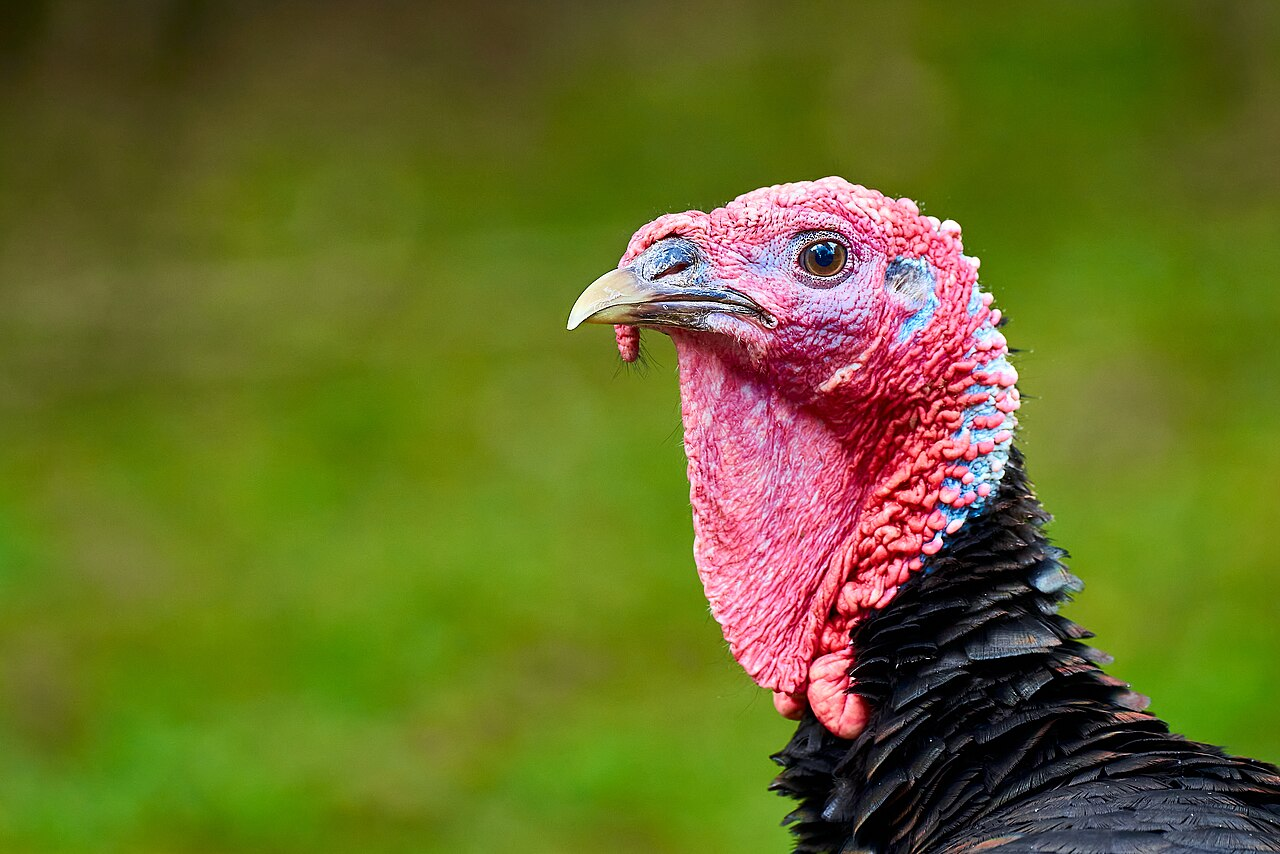
\includegraphics[width=\linewidth]{turkey.jpg}\\[0.15em]
      {\tiny\color{muted} A turkey. Photo: Anil \"Oztas, CC BY-SA 4.0\par}
    \end{column}
  \end{columns}
\end{frame}

\begin{frame}[plain]
  \vfill\centering
  {\fontsize{30}{36}\selectfont\bfseries\color{navy} What are you grateful for?\par}
  \vfill
\end{frame}

\photoframe{Why do we celebrate it?}{plymouth.jpg}{Jennie Augusta Brownscombe, \emph{Thanksgiving at Plymouth}. Public domain}

\photoframe{Macy's Thanksgiving Day Parade}{parade.jpg}{Inflating a balloon the night before the parade, New York. Photo: Rhododendrites, CC BY-SA 4.0}

\begin{frame}{Football}
  \begin{columns}[c,onlytextwidth]
    \begin{column}{0.49\textwidth}\centering
      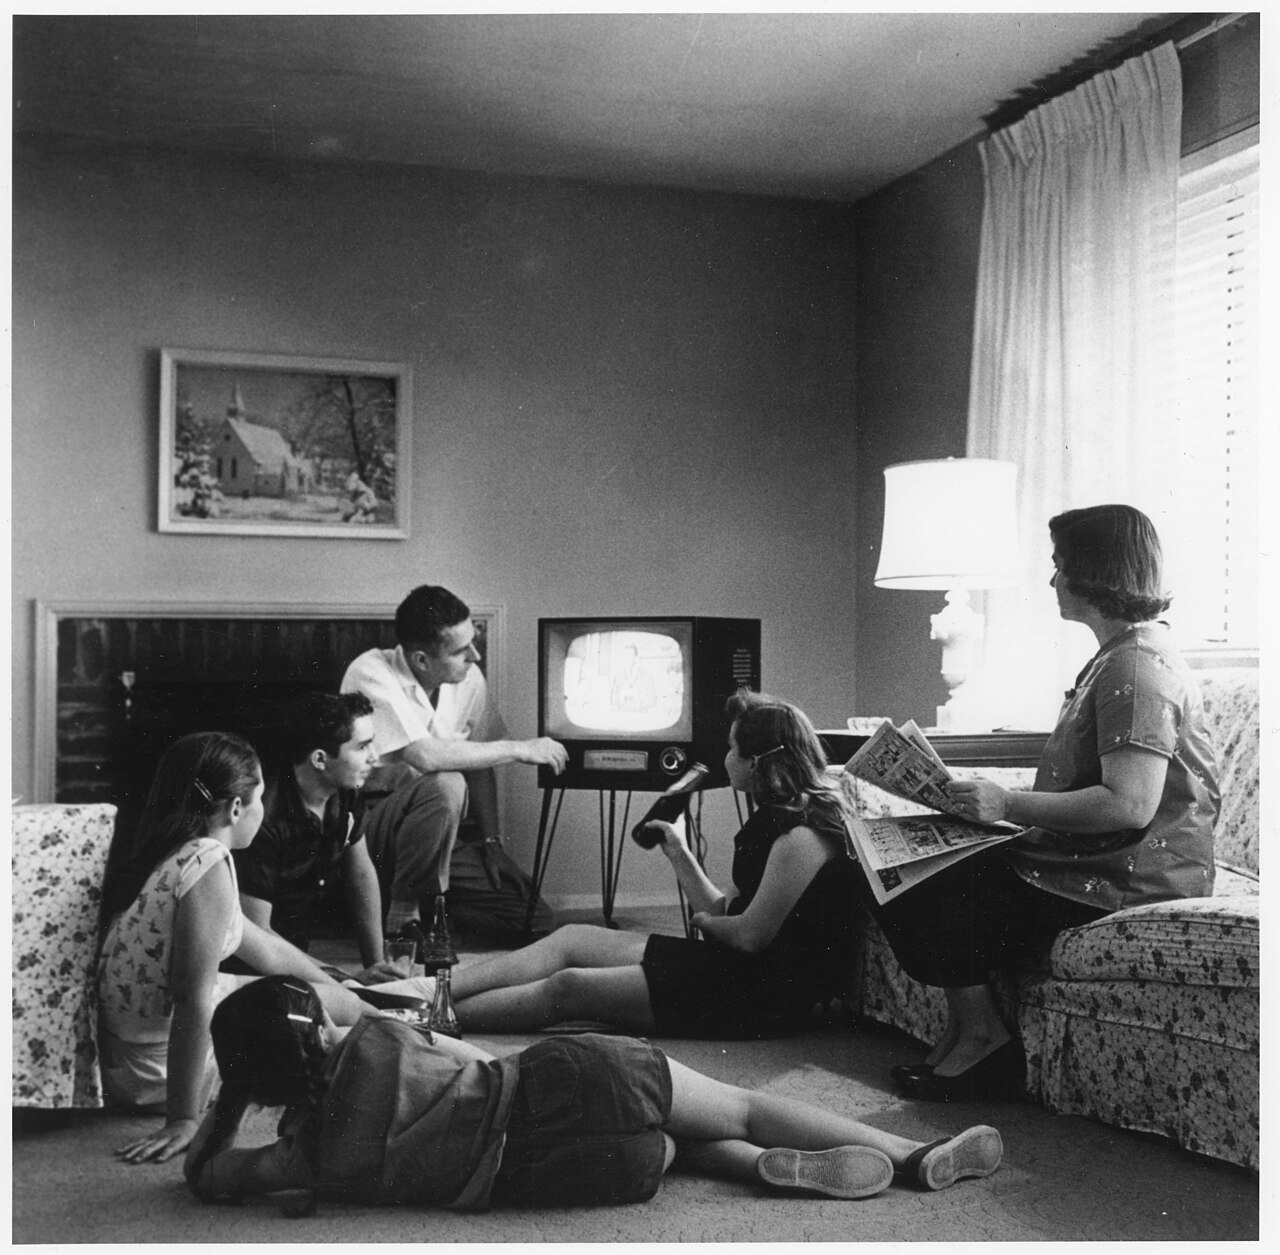
\includegraphics[width=\linewidth,height=0.58\paperheight,keepaspectratio]{tv1958.jpg}\\[0.15em]
      {\tiny\color{muted} An American family in front of the TV, 1958. Public domain\par}
    \end{column}
    \begin{column}{0.49\textwidth}\centering
      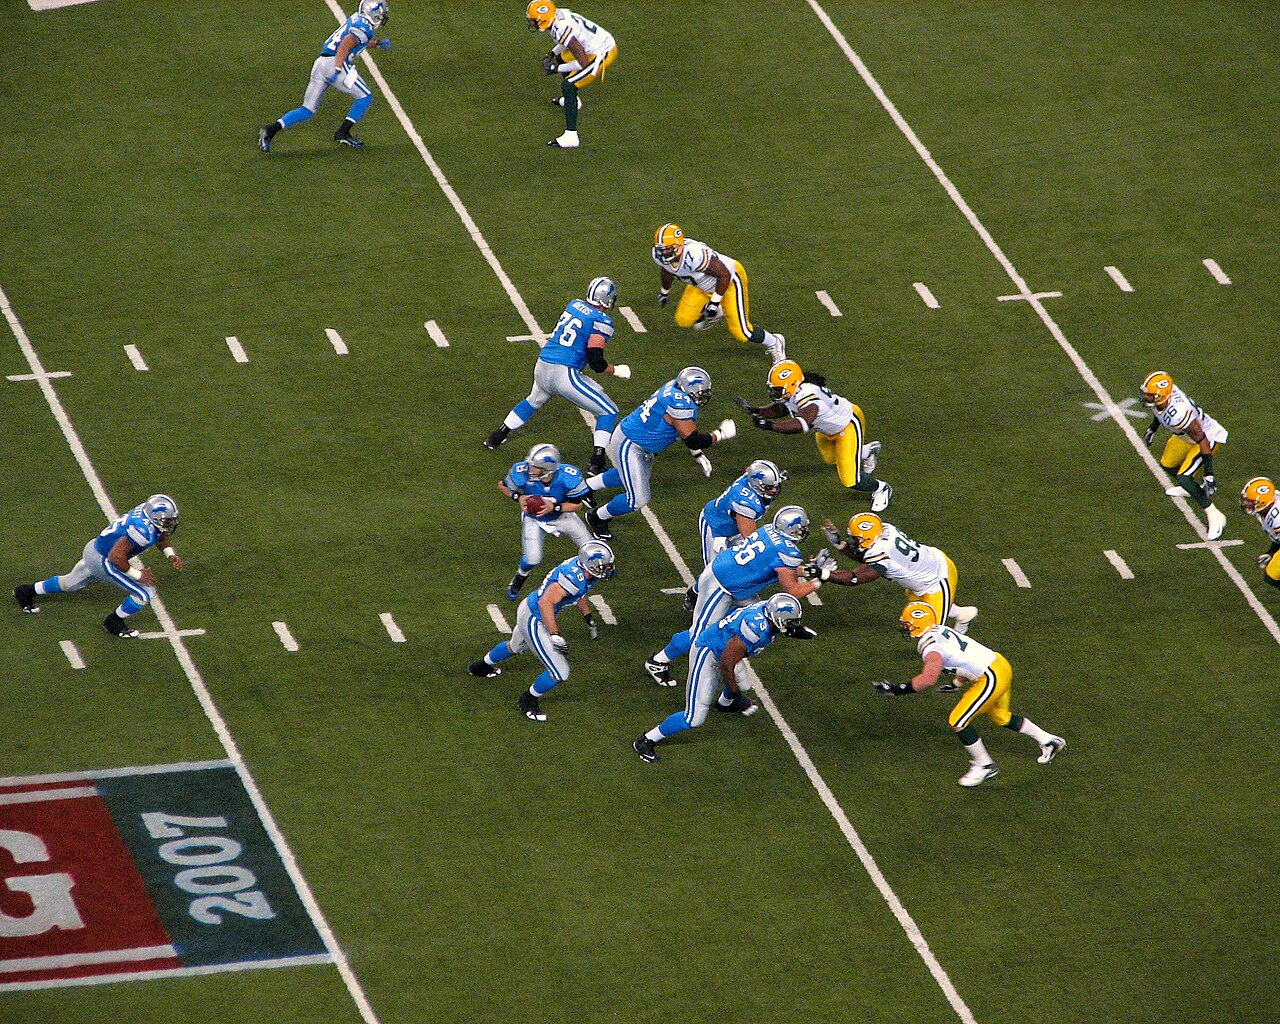
\includegraphics[width=\linewidth,height=0.58\paperheight,keepaspectratio]{football.jpg}\\[0.15em]
      {\tiny\color{muted} The Detroit Lions, Thanksgiving tradition since 1934. Photo: Dave Hogg, CC BY 2.0\par}
    \end{column}
  \end{columns}
\end{frame}

\begin{frame}{Guess!}
  \vfill\centering
  {\LARGE\bfseries How much weight does the average American\\[0.2em] gain over the holidays?\par}
  \vspace{1.6em}
  \onslide<2->{{\fontsize{34}{40}\selectfont\bfseries\color{oldred} 0.37 kg\par}\vspace{0.3em}{\large less than half a kilo\par}}
  \vfill
  \source{Source: Yanovski et al., \emph{New England Journal of Medicine} (2000). Thanksgiving to New Year.}
\end{frame}

% =====================================================================
\section{Thanksgiving Across America}

\whereframe{sauerkraut.jpg}{Photo: Alina Zienowicz, CC BY-SA 3.0}{Maryland}
\whereframe{kalua.jpg}{Kalua-style, slow-roasted Hawaiian way. Photo: Pacamah, CC BY 4.0}{Hawaii}
\whereframe{pecanpie.jpg}{Photo: Joe Hakim, CC BY 2.0}{The South}

\begin{frame}{Stuffing or dressing?}
  \begin{columns}[c,onlytextwidth]
    \begin{column}{0.56\textwidth}\centering
      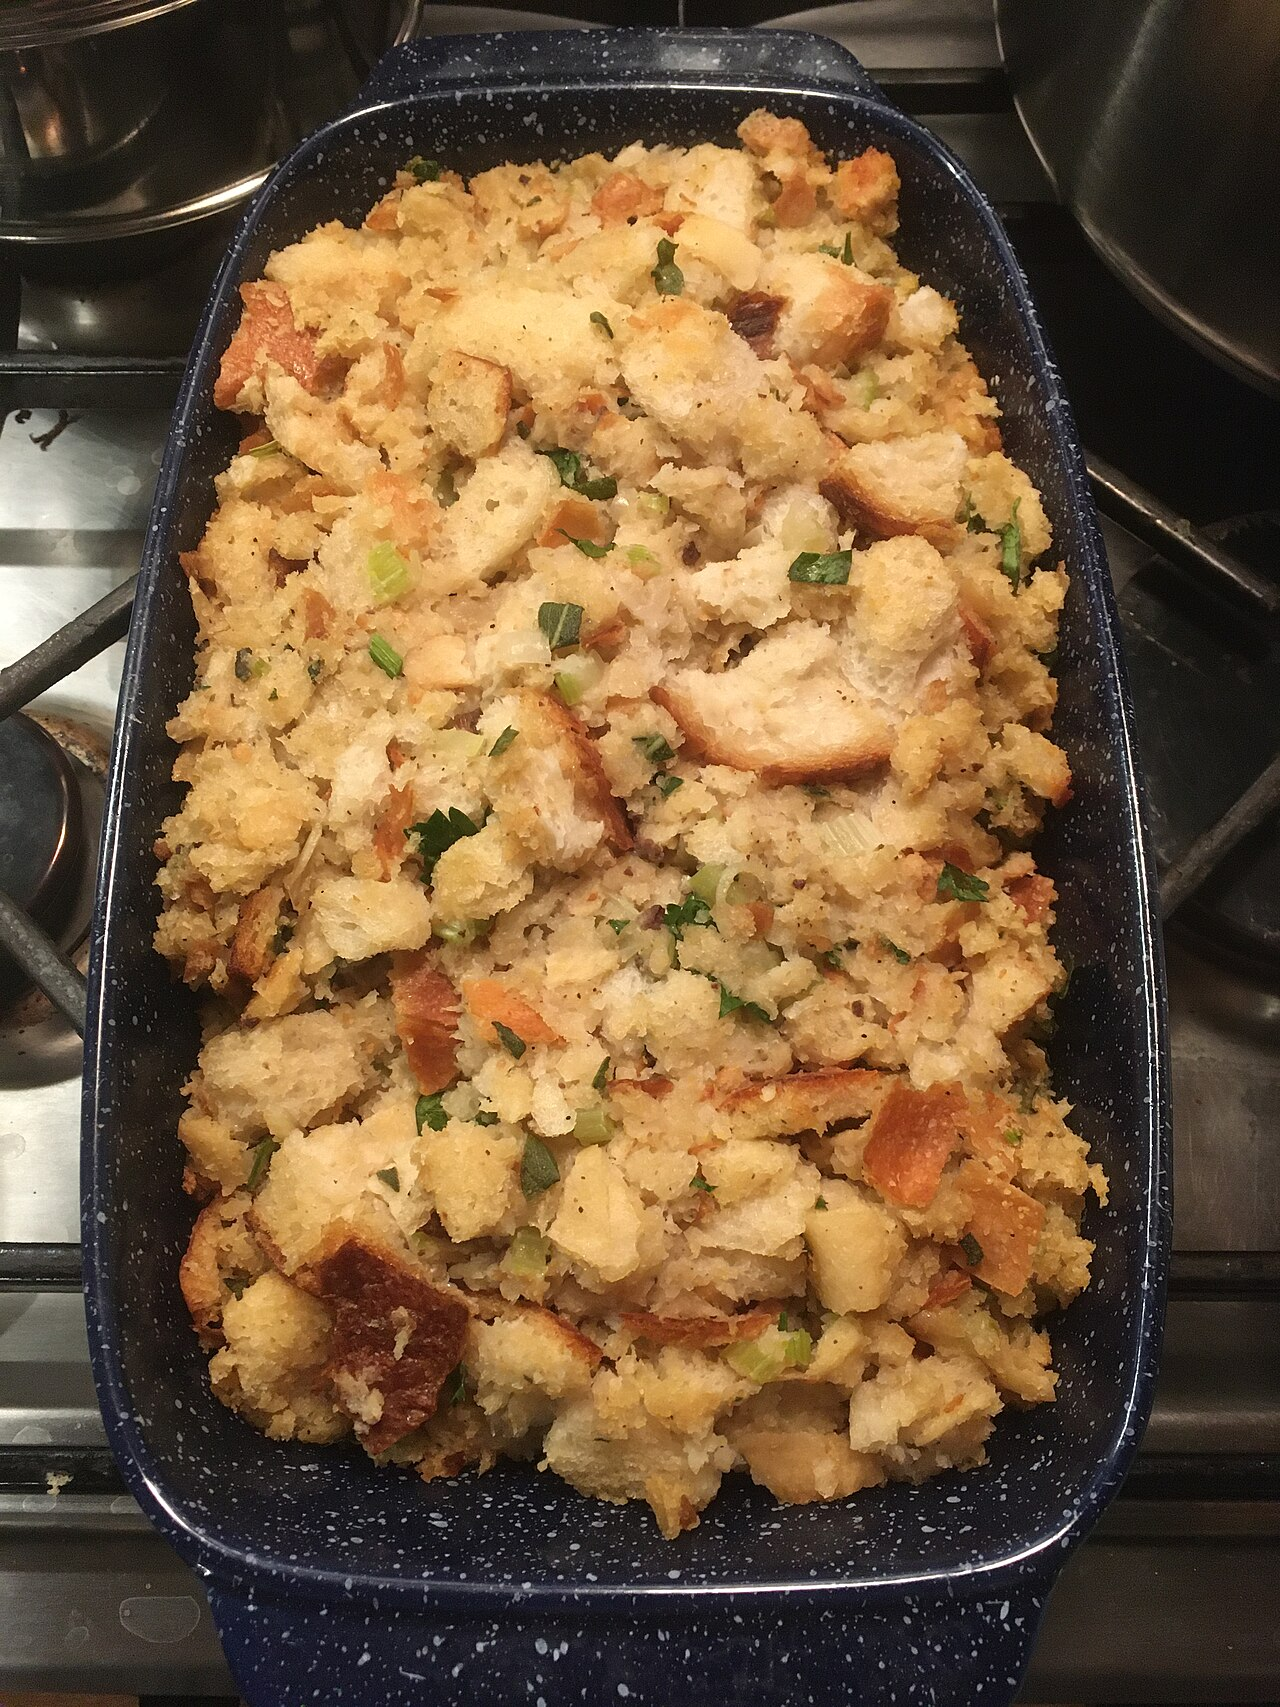
\includegraphics[width=\linewidth,height=0.6\paperheight,keepaspectratio]{stuffing.jpg}\\[0.15em]
      {\tiny\color{muted} Photo: Dorevabelfiore, CC BY-SA 4.0\par}
    \end{column}
    \begin{column}{0.4\textwidth}\centering
      \onslide<2->{{\Large The South:\par}{\fontsize{26}{32}\selectfont\bfseries\color{oldred} ``dressing''\par}\vspace{1.2em}}
      \onslide<3->{{\Large Everywhere else:\par}{\fontsize{26}{32}\selectfont\bfseries\color{oldblue} ``stuffing''\par}}
    \end{column}
  \end{columns}
  \source{Source: GE Appliances survey; Butterball survey (2015).}
\end{frame}

% =====================================================================
\section{Chopped! Thanksgiving Edition}

\begin{frame}{Chopped!}
  \begin{itemize}\setlength{\itemsep}{0.9em}\Large
    \item Four teams, four mystery baskets
    \item Use \alert{every} ingredient
    \item 10 minutes: plan one dish
    \item Pitch it to the judges
  \end{itemize}
\end{frame}

\basket{1}{roastturkey.jpg}{Turkey}{cranberry.jpg}{Canned cranberry sauce}{marshmallows.jpg}{Marshmallows}{pumpkinoil.jpg}{Pumpkin seed oil}
\basket{2}{sweetpotatoes.jpg}{Sweet potatoes}{pecans.jpg}{Pecans}{sauerkraut.jpg}{Sauerkraut}{candycorn.jpg}{Candy corn}
\basket{3}{pumpkin.jpg}{Pumpkin}{cornbread.jpg}{Cornbread}{wafers.jpg}{Wafers}{hotsauce.jpg}{Hot sauce}
\basket{4}{greenbeans.jpg}{Green beans}{friedonions.jpg}{Crispy fried onions}{maple.jpg}{Maple syrup}{cola.jpg}{Coca-Cola}

\begin{frame}{All four baskets}
  \centering
  \team{1}{roastturkey.jpg}{Turkey}{cranberry.jpg}{Cranberry sauce}{marshmallows.jpg}{Marshmallows}{pumpkinoil.jpg}{Pumpkin seed oil}\hfill
  \team{2}{sweetpotatoes.jpg}{Sweet potatoes}{pecans.jpg}{Pecans}{sauerkraut.jpg}{Sauerkraut}{candycorn.jpg}{Candy corn}\\[1.2em]
  \team{3}{pumpkin.jpg}{Pumpkin}{cornbread.jpg}{Cornbread}{wafers.jpg}{Wafers}{hotsauce.jpg}{Hot sauce}\hfill
  \team{4}{greenbeans.jpg}{Green beans}{friedonions.jpg}{Fried onions}{maple.jpg}{Maple syrup}{cola.jpg}{Coca-Cola}
  \source{Photos, Wikimedia Commons (CC BY, CC BY-SA, CC0, public domain): P.~Fitzgerald, Missvain, J.~Morgan, Kpjas, Melsj, R.~Culos, A.~Zienowicz, Evan-Amos, G.~Chernilevsky, Sherurcij, Samuel Wiki, T.~Harpel, G.~D.~Khadka, Famartin, M.~Andrade, O.~Yunakov.}
\end{frame}

\begin{frame}[plain]
  \begin{columns}[c,onlytextwidth]
    \begin{column}{0.47\textwidth}
      {\fontsize{28}{34}\selectfont\bfseries\color{navy} Happy\\Thanksgiving!\par}\vspace{0.6em}
      {\color{oldred}\rule{3cm}{1.5pt}}
    \end{column}
    \begin{column}{0.5\textwidth}
      \centering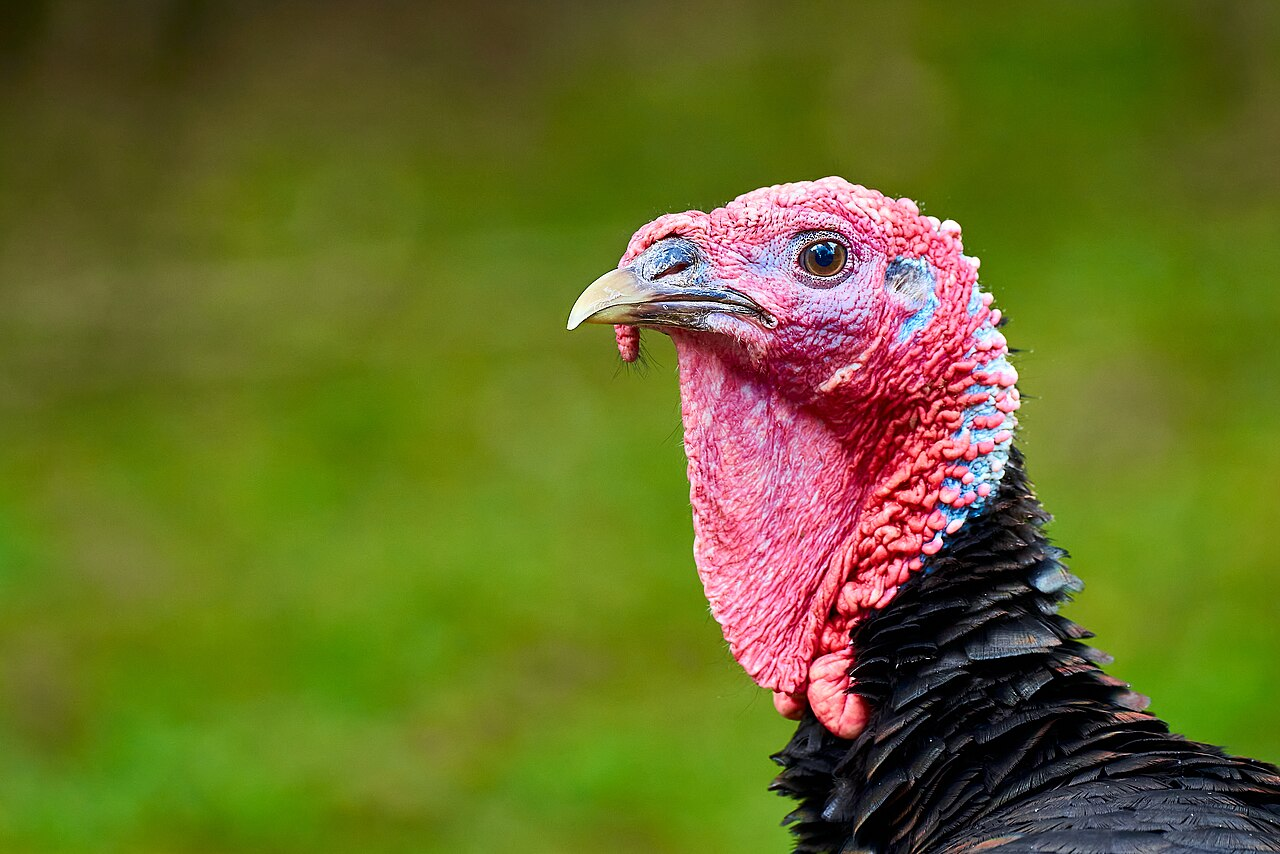
\includegraphics[width=\linewidth]{turkey.jpg}
    \end{column}
  \end{columns}
\end{frame}

\end{document}
